\chapter{Photon Polarization and the Logic of a Two-State System}

Quantum mechanics has already looked odd through interference and uncertainty, but in this lecture Susskind turns to a setting in which the oddness can be isolated with almost no technical overhead: the polarization of a photon. These notes follow Leonard Susskind's lecture closely, with explicit gratitude to Leonard Susskind, LazyingArt LLC, and Video2Book for the preserved lecture record from which the mathematical order and the blackboard evidence are reconstructed. The progression is the lecture's own: first the physical picture, then the symmetry puzzle, then the two-dimensional state space, then the enlargement from horizontal and vertical polarization to arbitrary angle, complex phase, and finally average value.

\section{Why Polarization Is the Right Starting Point}

The lecture opens by narrowing the photon to its simplest essential content. Let us imagine that the photon moves in a definite direction, say along the \(z\)-axis, with definite momentum. Then we are not discussing its motion at all; we are discussing only the remaining internal degree of freedom, namely polarization. In Susskind's language, the photon carries a little flag, and that flag lives in the plane perpendicular to the motion, the \(xy\)-plane.

\begin{figure}
\centering
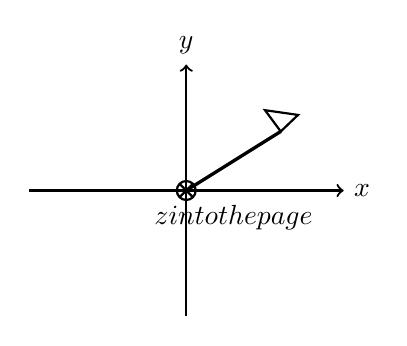
\begin{tikzpicture}[scale=1.0]
\draw[->,thick] (-2.0,0)--(2.0,0) node[right] {$x$};
\draw[->,thick] (0,-1.6)--(0,1.6) node[above] {$y$};
\draw[thick] (0,0) circle (0.12);
\draw[thick] (-0.08,-0.08)--(0.08,0.08);
\draw[thick] (-0.08,0.08)--(0.08,-0.08);
\draw[very thick] (0,0)--(1.2,0.75);
\draw[thick] (1.2,0.75)--(1.0,1.02)--(1.42,0.96)--cycle;
\draw (0.6,-0.35) node {$z\text{ into the page}$};
\end{tikzpicture}
\caption{A photon moving along the \(z\)-axis carries a transverse polarization ``flag'' in the \(xy\)-plane.}
\end{figure}

This is a physical picture, not yet a quantum formalism. It is useful precisely because it is so economical. We do not need the full machinery of particle motion; we need only one clean degree of freedom. The reward is that polarization gives us, in miniature, the logic of quantum mechanics itself.

At the same time Susskind is careful not to let the picture harden into naive classical language. We may say provisionally that the little flag points in some direction in the \(xy\)-plane, but the exact meaning of that sentence will only become clear after we translate the story into state vectors and observables. Before that translation, we first need to see how polarizers prepare and test the states.

\section{Classical Polarizers and the Quantum Tension}

A wire-grid polarizer is introduced only as far as the lecture needs it. The grid can support electric current in one direction but not in the orthogonal one. As a result, one component of the electric field is reflected and the perpendicular component passes through. Thus the grid prepares a transmitted wave polarized along a definite axis. It is that transmitted axis, not the grid lines themselves, that we use to label the polarizer.

\begin{figure}
\centering
\begin{tikzpicture}[scale=1.0]
\draw[thick] (0,-1)--(0,1);
\draw (0,-1.35) node {\(x\)};
\draw[thick,rotate around={90:(3,0)}] (3,-1)--(3,1);
\draw (3,-1.35) node {\(y\)};
\end{tikzpicture}
\caption{The horizontal and vertical polarizers that give the first two basis experiments.}
\end{figure}

Now send photons through one at a time. A horizontal polarizer prepares a photon in the horizontal state. If we place a second horizontal polarizer behind it, the photon goes through again. If we instead put a vertical polarizer behind the first, the photon does not go through. So a polarizer acts both as a preparer and as a measuring apparatus. It prepares a state when the photon passes, and it measures by pass-or-fail when the photon is tested by a later apparatus.

Up to this point there is nothing especially nonclassical. One could imagine bullets with little flags on them, together with an apparatus that lets one flag orientation through and blocks the other. The setup is deterministic. If the polarization matches the analyzer, the photon passes. If it does not, the photon is blocked, reflected, or absorbed. End of story.

But that is only the calm before the real difficulty. The lecture's explicit pivot is symmetry. If a polarizer may be held horizontally, and it may be held vertically, then rotational symmetry says it may be held at any intermediate angle. A photon can therefore be prepared with polarization axis at any direction in the \(xy\)-plane. Yet a fixed analyzer still produces only two outcomes: pass or fail. The photon is never chopped into pieces, partly transmitted and partly blocked. The outcomes are discrete even though the preparation angle varies continuously.

\subsection{Question \& Answer}

\paragraph{Question.}
If polarization can point in any direction, why does a fixed measurement still return only two outcomes?

\paragraph{Answer.}
That is the first real quantum question of the lecture. Continuity belongs to the space of possible preparations. Discreteness belongs to the outcome of a particular measurement. The classical picture tries to force both into the same mold, as if every intermediate polarization already carried a preexisting yes-or-no answer for every analyzer. Quantum mechanics does not do that. It assigns amplitudes to states, and a chosen analyzer converts those amplitudes into probabilities for its two possible outcomes.

This is why Susskind says the mystery begins here. We have a continuum of possible polarization states, but only two outcomes for any fixed polarizer. The tension between symmetry and discreteness is exactly what the two-dimensional quantum formalism must capture.

\section{The \(x\)-\(y\) Basis and the First Observable}

The lecture now restarts in a more formal register. We choose the simplest basis: horizontal and vertical polarization. Susskind labels them \(x\) and \(y\). Before he writes vectors, however, he pauses over a notation choice that matters conceptually. There is no distinction between horizontal polarization ``to the right'' and horizontal polarization ``to the left.'' A polarization axis is an axis, not a signed arrow. That is why he draws a double arrow.

\begin{figure}
\centering

\includegraphics[width=0.32\textwidth]{lecture_06_figure_02.png}
\par
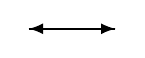
\begin{tikzpicture}[scale=1.0]
\draw[-latex,thick] (0,0)--(1.1,0);
\draw[-latex,thick] (1.1,0)--(0,0);
\end{tikzpicture}
\caption{Bidirectional mark for a polarization axis.}
\end{figure}

With that convention in hand, we define
\begin{equation}
|x\rangle=\begin{pmatrix}1\\0\end{pmatrix},
\qquad
|y\rangle=\begin{pmatrix}0\\1\end{pmatrix}.
\end{equation}
They are normalized and orthogonal:
\begin{equation}
\langle x|x\rangle=1,
\qquad
\langle y|y\rangle=1,
\qquad
\langle x|y\rangle=0.
\end{equation}
The space of states is therefore two-dimensional. That does not mean there are only two possible pure states; it means that every polarization state will be built from two basis vectors.

\begin{figure}
\centering

\includegraphics[width=0.55\textwidth]{lecture_06_figure_03.png}
\caption{Orthogonality and matrix action in the \(x,y\) basis.}
\end{figure}

The blackboard fragment above is useful precisely because it preserves the board layout: orthogonality at upper left, operator action in the main field. The visible multiplication is
\begin{equation}
\begin{pmatrix}
1&0\\
0&-1
\end{pmatrix}
\begin{pmatrix}
1\\
0
\end{pmatrix},
\end{equation}
and the standard continuation of that displayed step is
\begin{equation}
\begin{pmatrix}
1&0\\
0&-1
\end{pmatrix}
\begin{pmatrix}
1\\
0
\end{pmatrix}
=
\begin{pmatrix}
1\\
0
\end{pmatrix}.
\end{equation}

The first observable is built directly from the measuring procedure. Send the photon through an \(x\)-polarizer. Record \(+1\) if it passes and \(-1\) if it does not. Those numbers are conventional; Susskind emphasizes that we could have chosen others. But \(\pm1\) are natural. The operator is defined by
\begin{equation}
\hat P_{xy}|x\rangle=+|x\rangle,
\qquad
\hat P_{xy}|y\rangle=-|y\rangle.
\end{equation}
In the \((|x\rangle,|y\rangle)\) basis this means
\begin{equation}
P_{xy}=
\begin{pmatrix}
1&0\\
0&-1
\end{pmatrix}.
\end{equation}

This is the first concrete example of the general postulate. An observable is represented by an operator. Its eigenvectors are the states in which the observable is definite, and its eigenvalues are the definite outcomes. The language is abstract, but the content here is still very physical: pass gives \(+1\), fail gives \(-1\).

\section{From \(45^\circ\) to Arbitrary Angles}

The lecture now extends the basis in the most controlled way possible. What if we rotate the polarizer by \(45^\circ\)? The outgoing state is neither \(|x\rangle\) nor \(|y\rangle\). Since it lies halfway between the two axes, it is natural that it have equal probabilities to pass an \(x\)-analyzer and a \(y\)-analyzer. This motivates
\begin{equation}
|/\rangle=\frac{1}{\sqrt2}\bigl(|x\rangle+|y\rangle\bigr)
=
\frac{1}{\sqrt2}
\begin{pmatrix}
1\\
1
\end{pmatrix}.
\end{equation}
Its orthogonal companion may be taken as
\begin{equation}
|\backslash\rangle=\frac{1}{\sqrt2}\bigl(|x\rangle-|y\rangle\bigr)
=
\frac{1}{\sqrt2}
\begin{pmatrix}
1\\
-1
\end{pmatrix}.
\end{equation}
The overall sign is inessential; one could equally well put the minus sign on the first component. What matters is orthogonality:
\begin{equation}
\langle /|\backslash\rangle=\frac12-\frac12=0.
\end{equation}

\begin{figure}
\centering
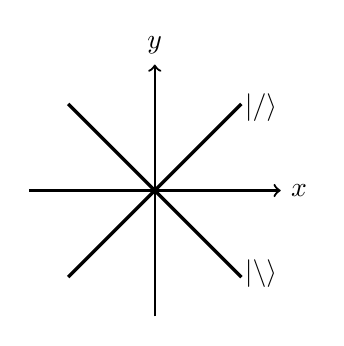
\begin{tikzpicture}[scale=1.0]
\draw[->,thick] (-1.6,0)--(1.6,0) node[right] {$x$};
\draw[->,thick] (0,-1.6)--(0,1.6) node[above] {$y$};
\draw[very thick] (-1.1,-1.1)--(1.1,1.1);
\draw[very thick] (-1.1,1.1)--(1.1,-1.1);
\draw (1.35,1.05) node {\(|/\rangle\)};
\draw (1.35,-1.05) node {\(|\backslash\rangle\)};
\end{tikzpicture}
\caption{The slash and backslash polarization axes, rotated by \(45^\circ\) with respect to the \(x,y\) basis.}
\end{figure}

The measurement rule now shows its first genuinely quantum face. The amplitude to find the photon in the \(x\)-state is
\begin{equation}
\langle x|/\rangle=\frac{1}{\sqrt2},
\end{equation}
so the probability that a slash-polarized photon passes an \(x\)-polarizer is
\begin{equation}
|\langle x|/\rangle|^2=\frac12.
\end{equation}
Likewise
\begin{equation}
|\langle y|/\rangle|^2=\frac12.
\end{equation}

Now we may ask for the observable that is definite in the slash/backslash basis. The transcript is visibly garbled at the moment the matrix is written, so the clean matrix must be presented cautiously. The natural reconstruction, and the unique symmetric matrix consistent with the stated eigenvalue equations, is
\begin{equation}
P_{/\backslash}=
\begin{pmatrix}
0&1\\
1&0
\end{pmatrix},
\end{equation}
since
\begin{align}
P_{/\backslash}
\begin{pmatrix}
1\\
1
\end{pmatrix}
&=
\begin{pmatrix}
1\\
1
\end{pmatrix},
&
P_{/\backslash}
\begin{pmatrix}
1\\
-1
\end{pmatrix}
&=
-
\begin{pmatrix}
1\\
-1
\end{pmatrix}.
\end{align}

This is also the moment at which Susskind cleans up a conceptual point that is easy to lose. A state does not tell us what is observable; everything represented by an observable is observable. A state tells us what is definite. In the slash state, the slash/backslash observable is definite, but the original \(x,y\) observable is only probabilistic.

From here the lecture proceeds to an arbitrary angle \(\theta\). If the polarization axis is rotated by \(\theta\) from horizontal, the corresponding unit vector has components \(\cos\theta\) and \(\sin\theta\). Thus
\begin{equation}
|\theta\rangle=\cos\theta\,|x\rangle+\sin\theta\,|y\rangle
=
\begin{pmatrix}
\cos\theta\\
\sin\theta
\end{pmatrix}.
\end{equation}
The orthogonal companion is the state at \(\theta+\pi/2\):
\begin{equation}
|\theta+\pi/2\rangle
=
-\sin\theta\,|x\rangle+\cos\theta\,|y\rangle
=
\begin{pmatrix}
-\sin\theta\\
\cos\theta
\end{pmatrix}.
\end{equation}
These are normalized because \(\cos^2\theta+\sin^2\theta=1\), and orthogonal because
\begin{equation}
\langle\theta|\theta+\pi/2\rangle
=
\cos\theta(-\sin\theta)+\sin\theta\cos\theta
=
0.
\end{equation}

Now we ask the experimental question that quantum mechanics is built to answer. A photon emerges from a \(\theta\)-polarizer. What is the probability that it passes an \(x\)-polarizer? The amplitude is
\begin{equation}
\langle x|\theta\rangle=\cos\theta,
\end{equation}
so
\begin{equation}
P(\theta\to x)=|\langle x|\theta\rangle|^2=\cos^2\theta.
\end{equation}
Likewise
\begin{equation}
P(\theta\to y)=|\langle y|\theta\rangle|^2=\sin^2\theta,
\end{equation}
and the total probability is \(1\).

\paragraph{Trigonometric interlude.}
At this point the lecture pauses for a small table of trigonometric identities, not as a digression but because the general two-polarizer experiment now demands them:
\begin{align}
\cos(\alpha+\beta)&=\cos\alpha\cos\beta-\sin\alpha\sin\beta,\\
\cos(\alpha-\beta)&=\cos\alpha\cos\beta+\sin\alpha\sin\beta,\\
\sin(\alpha+\beta)&=\sin\alpha\cos\beta+\sin\beta\cos\alpha,\\
\sin(\alpha-\beta)&=\sin\alpha\cos\beta-\sin\beta\cos\alpha,\\
\cos 2\alpha&=\cos^2\alpha-\sin^2\alpha,\\
\sin 2\alpha&=2\sin\alpha\cos\alpha.
\end{align}

\begin{figure}
\centering
\begin{tikzpicture}[scale=1.0]
\draw[->,thick] (-0.8,0)--(7.8,0);
\draw[thick,rotate around={25:(1,0)}] (1,-1)--(1,1);
\draw[thick,rotate around={70:(5,0)}] (5,-1)--(5,1);
\draw (1,-1.35) node {$\alpha$};
\draw (5,-1.35) node {$\beta$};
\draw (3.0,0.45) node {$|\alpha\rangle$};
\end{tikzpicture}
\caption{A photon prepared by an \(\alpha\)-polarizer and tested by a second polarizer at angle \(\beta\).}
\end{figure}

If the first polarizer prepares
\begin{equation}
|\alpha\rangle=
\begin{pmatrix}
\cos\alpha\\
\sin\alpha
\end{pmatrix},
\qquad
\langle \beta|=
\begin{pmatrix}
\cos\beta&\sin\beta
\end{pmatrix},
\end{equation}
then the amplitude to pass the second polarizer is
\begin{equation}
\langle\beta|\alpha\rangle
=
\cos\alpha\cos\beta+\sin\alpha\sin\beta
=
\cos(\alpha-\beta).
\end{equation}
This is not yet the probability. The lecture makes a point of this: the quantity can be negative, so it cannot itself be a probability. The transmission probability is the square of the amplitude,
\begin{equation}
P(\alpha\to\beta)=|\langle\beta|\alpha\rangle|^2=\cos^2(\alpha-\beta).
\end{equation}
The answer depends only on the relative angle, as symmetry says it must, and yet the actual outcome of each trial remains one of two discrete possibilities. This is exactly the pattern the lecture set out to display.

\section{Intermediate Polarizers and the Observable \(P_\theta\)}

After the break the lecture reopens not with a new theorem but with a puzzle raised by students. That is the right rhythm for the notes as well.

\subsection{Question \& Answer}

\paragraph{Question.}
How can adding another polarizer increase the chance of transmission?

\paragraph{Answer.}
Suppose a photon has passed a \(\theta\)-polarizer, so it is in the state \(|\theta\rangle\). If we test it immediately with a \(\theta+\pi/2\) polarizer, the probability of transmission is
\begin{equation}
P(\theta\to \theta+\pi/2)=\cos^2(\pi/2)=0.
\end{equation}
The direct channel is completely closed.

Now insert a horizontal polarizer in between. First the photon must pass the middle polarizer:
\begin{equation}
P(\theta\to x)=\cos^2\theta.
\end{equation}
But if it does pass, the state has changed. It is no longer \(|\theta\rangle\); it has been prepared anew as \(|x\rangle\). The probability that this new state passes the final polarizer is therefore
\begin{equation}
P(x\to \theta+\pi/2)=\sin^2\theta.
\end{equation}
Hence the total probability is not an addition but a product of successive conditional probabilities:
\begin{equation}
P(\theta\to x\to \theta+\pi/2)=\cos^2\theta\,\sin^2\theta.
\end{equation}

\begin{figure}
\centering
\begin{tikzpicture}[scale=1.0]
\draw[->,thick] (-0.8,0)--(8.8,0);
\draw[thick,rotate around={30:(1,0)}] (1,-1)--(1,1);
\draw[thick] (4,-1)--(4,1);
\draw[thick,rotate around={120:(7,0)}] (7,-1)--(7,1);
\draw (1,-1.35) node {$\theta$};
\draw (4,-1.35) node {$x$};
\draw (7,-1.55) node {$\theta+\pi/2$};
\end{tikzpicture}
\caption{The inserted horizontal polarizer prepares a new state. That is why the forbidden direct channel can reopen with nonzero probability.}
\end{figure}

The surprise is not that extra apparatus creates photons that were not there. The surprise is that measurement changes the state. By inserting a polarizer in between, we do not merely diminish an existing channel; we alter the state on which the next analyzer acts. That is why Susskind calls this one of the mildly freaky interference phenomena.

The lecture then returns to the general observable \(\hat P_\theta\). Here Susskind is candid: solving for the matrix component by component is not very illuminating, but seeing the answer and checking it is reassuring. We want an operator with
\begin{equation}
\hat P_\theta|\theta\rangle=+|\theta\rangle,
\qquad
\hat P_\theta|\theta+\pi/2\rangle=-|\theta+\pi/2\rangle.
\end{equation}
The transcript is partially garbled where the matrix is first written, but the cleaned result is standard and fully consistent with the stated eigenvalue equations:
\begin{equation}
P_\theta=
\begin{pmatrix}
\cos 2\theta & \sin 2\theta\\
\sin 2\theta & -\cos 2\theta
\end{pmatrix}.
\end{equation}

To check it, set
\begin{equation}
c=\cos\theta,
\qquad
s=\sin\theta,
\qquad
|\theta\rangle=
\begin{pmatrix}
c\\
s
\end{pmatrix}.
\end{equation}
Then
\begin{align}
P_\theta|\theta\rangle
&=
\begin{pmatrix}
c^2-s^2 & 2sc\\
2sc & s^2-c^2
\end{pmatrix}
\begin{pmatrix}
c\\
s
\end{pmatrix} \\
&=
\begin{pmatrix}
(c^2-s^2)c+2sc\,s\\
2sc\,c+(s^2-c^2)s
\end{pmatrix} \\
&=
\begin{pmatrix}
c(c^2+s^2)\\
s(c^2+s^2)
\end{pmatrix}
=
\begin{pmatrix}
c\\
s
\end{pmatrix}
=
|\theta\rangle.
\end{align}
The companion vector \(|\theta+\pi/2\rangle\) is similarly sent to minus itself. Thus the matrix has exactly the required eigenvectors and eigenvalues.

The \(90^\circ\) rotation now has a clean operator statement:
\begin{equation}
P_{\theta+\pi/2}=-P_\theta.
\end{equation}
That is just the exchange of the positive and negative eigenvalues. The orthogonal analyzer does not introduce a wholly different observable; it flips the sign convention for the same pair of eigenstates.

\section{Complex Coefficients and Circular Polarization}

At this point Susskind widens the state space one more time. We have not yet used complex numbers, and quantum mechanics is built from them. So we introduce a new state,
\begin{equation}
|c_+\rangle=\frac{1}{\sqrt2}
\begin{pmatrix}
1\\
i
\end{pmatrix},
\end{equation}
together with its orthogonal partner
\begin{equation}
|c_-\rangle=\frac{1}{\sqrt2}
\begin{pmatrix}
1\\
-i
\end{pmatrix}.
\end{equation}
Normalization requires complex conjugation:
\begin{equation}
\langle c_+|c_+\rangle
=
\frac12\bigl(1\cdot 1+(-i)\cdot i\bigr)=1.
\end{equation}
Orthogonality does too:
\begin{equation}
\langle c_-|c_+\rangle
=
\frac12\bigl(1\cdot 1+i\cdot i\bigr)=0.
\end{equation}
This is a point the lecture emphasizes strongly. If we forget the bra and simply dot the columns together, we get the wrong answer. The bra is already the complex-conjugated object.

From the wave point of view, these states correspond to a phase difference between the \(x\)- and \(y\)-components of the electric field. If
\begin{equation}
E_y=\cos(z-ct),
\qquad
E_x=\cos(z-ct),
\end{equation}
then the two components are in phase and the result is just linear polarization at \(45^\circ\). Circular polarization appears when the components are out of phase by \(90^\circ\):
\begin{equation}
E_y=\cos(z-ct),
\qquad
E_x=\sin(z-ct),
\end{equation}
or with the opposite sign in the second equation. At a fixed point in space the electric field rotates in time. That is the wave picture behind the complex state vector.

The lecture informally calls the two states left and right circular polarization, but Susskind explicitly remarks that he may have the handedness labels mixed up. The important thing for us is the pair of states \(\frac1{\sqrt2}(1,\pm i)^T\), not the convention for the names.

Now test a circularly polarized photon with a linear polarizer at angle \(\theta\). Since
\begin{equation}
|\theta\rangle=
\begin{pmatrix}
\cos\theta\\
\sin\theta
\end{pmatrix},
\end{equation}
the amplitude is
\begin{equation}
\langle\theta|c_+\rangle
=
\frac{1}{\sqrt2}\bigl(\cos\theta+i\sin\theta\bigr).
\end{equation}
The probability is the modulus squared,
\begin{align}
|\langle\theta|c_+\rangle|^2
&=
\frac12\bigl(\cos\theta+i\sin\theta\bigr)\bigl(\cos\theta-i\sin\theta\bigr) \\
&=
\frac12\bigl(\cos^2\theta+\sin^2\theta\bigr)
=
\frac12.
\end{align}
So a circularly polarized photon passes any linearly polarized analyzer with probability \(1/2\). That is the precise fact the lecture uses. Beyond that lies the wider family of elliptically polarized states, but Susskind only gestures toward them here and postpones the corresponding observables.

A quarter-wave plate is mentioned as the device that produces circular polarization by shifting the two linear components out of phase. The details are left for the next lecture, which is exactly right: the mathematical point needed here is only that complex phase opens new states which are not visible in the real two-parameter picture of linear polarization alone.

\section{Incompatible Observables and Average Value}

By now we have a whole family of polarization observables: horizontal/vertical, slash/backslash, the general \(P_\theta\), and a circular observable left as homework. The common structural fact is that different polarization observables generally do not commute. The reason is already visible at the level of eigenvectors. Horizontal and vertical states are one basis. Slash and backslash are another. Circular states are a third. In general they do not share eigenvectors, so they are not simultaneously definite.

The special case is the orthogonal pair \(\theta\) and \(\theta+\pi/2\). Their observables are just negatives of each other:
\begin{equation}
P_{\theta+\pi/2}=-P_\theta.
\end{equation}
Therefore they commute. Measuring one automatically tells us the other, since the eigenvalue has simply changed sign. But for genuinely different angles, or for linear versus circular polarization, the observables are incompatible. One cannot have a polarizer that prepares definite \(x\)-polarization and definite \(\theta\)-polarization at the same time.

The lecture now makes its final pivot. We have been calculating probabilities. What about average value? Susskind immediately objects to the standard terminology. ``Expectation value'' is, he says, a poor choice of words, because it often names the last value one should expect to see in a single trial.

\begin{figure}
\centering

\includegraphics[width=0.58\textwidth]{lecture_06_figure_04.png}
\par
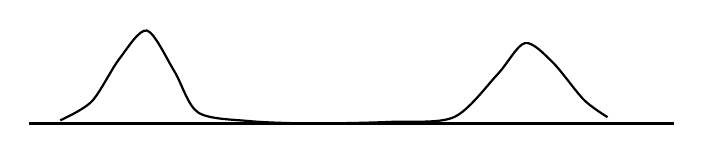
\begin{tikzpicture}[scale=1.0]
\draw[thick] (-4.1,0)--(4.1,0);
\draw[thick,smooth] plot coordinates {
(-3.7,0.04) (-3.3,0.28) (-2.95,0.82) (-2.6,1.18) (-2.25,0.66)
(-1.95,0.14) (-1.3,0.03) (-0.5,0.00) (0.5,0.02) (1.3,0.08)
(1.85,0.62) (2.2,1.02) (2.55,0.78) (2.95,0.30) (3.25,0.08)};
\end{tikzpicture}
\caption{Symmetric two-lump wavefunction profile.}
\end{figure}

The sketch above carries no algebra on the board, but it carries the geometry of the example. A symmetric wavefunction with one lump on the left and one on the right has
\begin{equation}
\langle x\rangle=0,
\end{equation}
yet the particle is least likely to be found at the middle. So the expectation value is not the value one should expect to observe on a single shot. It is an average value.

Now let \(K\) be any Hermitian observable with eigenvectors \(|n\rangle\) and eigenvalues \(\lambda_n\):
\begin{equation}
K|n\rangle=\lambda_n|n\rangle.
\end{equation}
If \(|\psi\rangle\) is any state, define the average value by the sandwich
\begin{equation}
\langle K\rangle_\psi=\langle\psi|K|\psi\rangle.
\end{equation}
There is no extra star on \(K\); the bra already carries the complex conjugation. Insert the identity in the form
\begin{equation}
\sum_n |n\rangle\langle n|=I.
\end{equation}
Then
\begin{align}
\langle K\rangle_\psi
&=
\langle\psi|K|\psi\rangle \\
&=
\left\langle\psi\left|K\left(\sum_n |n\rangle\langle n|\right)\right|\psi\right\rangle \\
&=
\sum_n \langle\psi|K|n\rangle\langle n|\psi\rangle \\
&=
\sum_n \lambda_n\,\langle\psi|n\rangle\langle n|\psi\rangle \\
&=
\sum_n \lambda_n\,|\langle n|\psi\rangle|^2.
\end{align}
This is exactly the ordinary weighted average of all possible outcomes: eigenvalue times probability, summed over the basis of outcomes.

For polarization the simplest example uses the original operator \(P_{xy}\) in the state \(|\theta\rangle\):
\begin{align}
\langle P_{xy}\rangle_\theta
&=
\langle\theta|P_{xy}|\theta\rangle \\
&=
\begin{pmatrix}
\cos\theta & \sin\theta
\end{pmatrix}
\begin{pmatrix}
1&0\\
0&-1
\end{pmatrix}
\begin{pmatrix}
\cos\theta\\
\sin\theta
\end{pmatrix} \\
&=
\cos^2\theta-\sin^2\theta \\
&=
\cos 2\theta.
\end{align}
This lies between \(+1\) and \(-1\), as it should. But again, it is not a new measurement outcome. The actual outcomes are still \(+1\) and \(-1\). The quantity \(\cos 2\theta\) is their average over many repetitions.

\section{Summary}

Polarization is the right starting point because it is small enough to see clearly and rich enough to contain the full logical structure of quantum mechanics. We begin with a photon moving along \(z\), carrying a transverse flag in the \(xy\)-plane. We then discover the central tension: symmetry allows a continuum of preparation directions, but every fixed analyzer still returns only two outcomes. From that point the lecture unfolds methodically. We choose a basis, construct observables, rotate the basis, extract amplitudes and probabilities, see how measurements update the state, admit complex phase and circular polarization, and finally learn to distinguish a probability from an average value. The system is minimal, but the logic is already complete.